\chapter{Design}

\section{User Context}
During the authentication process, the crucial part to successfully authenticate user is to get information about multiple authentication factors, as described in the section \ref{authentication-factors}.
It is an essential part of security strengthening as the more information we get from the authentication attempt, the more we can react to it and evaluate it.

User context is a concept that represents a piece of information about the authentication attempt, such as current device attributes, information about the user, location, or behavior we detected.
Even though the information about the device does not seem to reflect the term user context, it should be considered like it.
User context represents the information about the user of the application, even when it is a service account, for instance.

During the authentication process, user contexts are always collected and grouped into a more comprehensive knowledge base.
The proper user context management is a crucial part of the authentication, especially for the risk-based authentication mechanism.

The abstraction around fetching user contexts provides the ability to easily extend and process possible user context information and gives the freedom to obtain various types of contexts, even from remote locations.

The main advantage of using user contexts is to get the required information, regardless of the source of the information.
It means that it does not really matter which approach was used for obtaining the information, but that the information is available.
It implies that administrators need to be aware of present user context providers/implementations in order to prevent any inaccuracies.

\newpage

As shown in Figure \ref{fig:user-context-diagram}, user context is represented as interface \textit{UserContext}, where the generic is used.
It means that every implementation of the \textit{UserContext} interface can retrieve different type of data.

\begin{figure}[htbp]
  \centering
  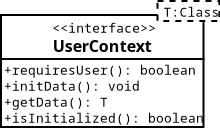
\includegraphics[width=0.4\textwidth]{img/sections/5-design/userContext.png}
  \label{fig:user-context-diagram}
  \caption{User Context Diagram}
\end{figure}

Methods of the \textit{UserContext} interface:
\begin{itemize}
    \item \textit{requiresUser()} -- a boolean flag to determine whether the data can be obtained without the information about the authentication user.
    \item \textit{initData()} -- method that initiates retrieving the data.
    \item \textit{getData()} -- obtain the retrieved data. 
    \item \textit{isInitialized()} -- a boolean flag to determine whether the data is already initialized. 
\end{itemize}

\newpage

\subsection{Specific User Context}
An excellent example of leveraging user context is the implementation of an IP address context.
It provides the ability to obtain the IP address of the device in multiple ways.
The IP address can be obtained either from the user agent attributes or from the HTTP headers 'Forwarded' and 'X-Forwarded-For' when a proxy is used.

As you can see in Figure \ref{fig:user-context-ip-address-context}, the \textit{IpAddressContext} interface extends the \textit{UserContext} interface and specify that the retrieved data will be of type \textit{IPAddress}, which is a structure describing the IP address attributes.

The \textit{DeviceIpAddressContext} class is an implementation of the \textit{IpAddressContext} interface and obtains the IP address from the user agent attributes.
The \textit{HeaderIpAddressContext} class is also an implementation of the \textit{IpAddressContext} interface and obtains the IP address from the HTTP headers, when a proxy is used.

\begin{figure}[htbp]
  \centering
  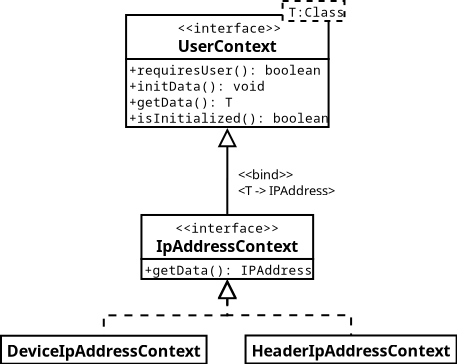
\includegraphics[width=0.8\textwidth]{img/sections/5-design/ipAddressContext.png}
  \label{fig:user-context-ip-address-context}
  \caption{IP Address User Context Diagram}
\end{figure}

\subsection{User Context Condition}
Improvement to the user context management is to have a general concept for evaluating certain conditions with regard to the user context.
It means that we can leverage user context conditions in conditional authentication flows or in authentication policies, as described in \ref{authentication-policies}.

There might be several possible operations make on the user context entities, and the developer of the additional user context should not reinvent the wheel around attributes of conditions.
The additional conditions can be created very easily, as the general concept for evaluating them has already been assessed.

The abstract \textit{UserContextConditionFactory} class implements the \textit{VerifiableUserContextFactory} interface, that manages the \textit{Operation} class described in the section \ref{user-context-condition-operations}.

\begin{figure}[htbp]
  \centering
  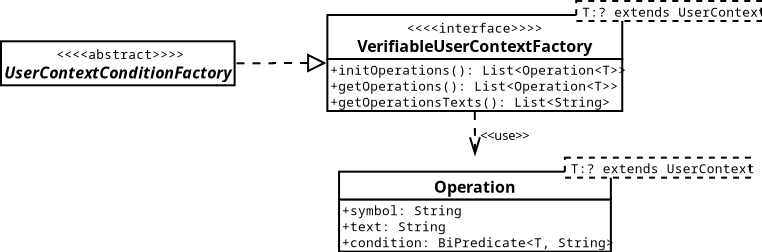
\includegraphics[width=1\textwidth]{img/sections/5-design/UserContextCondition.png}
  \label{fig:user-context-condition}
  \caption{User Context Condition Diagram}
\end{figure}

\subsubsection{Operations} \label{user-context-condition-operations}
User context conditions take into account a list of operations that can be proceeded on the user context entity.
The operation consists of several attributes, such as follows:

\begin{itemize}
    \item \textbf{Symbol} (\textit{string}) -- unique operation identifier used for identification of the operation when serialized data are received from remote locations. It must be unique per the user context condition.
    \item \textbf{Text} (\textit{string}) -- name of the operation shown to the end user.
    It can contain a localization key, which can then be mapped to a different language or directly the text in the specific language. 
    \item \textbf{Predicate} (\textit{predicate}) -- predicate that is applied to the specific user context. When the evaluation of the predicate is met, the operation is considered successful.
\end{itemize}

When all the predicates of specified operations are met, the whole condition is considered successful, and the authentication flow can proceed with the processing.

\subsubsection{Example}

A suitable example of the user context condition might be a newly introduced condition for the IP address user context entity.
During the evaluation of the condition, the first step is obtaining the IP address context, which contains the current IP address of the device that is trying to authenticate.
Some specified operations that can be made on top of the IP address context are `is equal`, `is not equal` or `is in range`.

The predicate of the \textit{equal} operation is to directly match the IP address provided by the administrator.
The opposite \textit{not equal} operation just negatively matches the IP address, as it represents the state when the IP address is not the specified one.
Administrators can also specify the `in range` operation, which provides the ability to check whether the IP address of the device is in the specified IP address range.

For instance, an administrator can specify that IP addresses from the range `222.0.0.0-224.0.0.0` are not allowed to be authenticated, as shown in Figure \ref{fig:design-user-context-ip-addr-condition}.

\begin{figure}[htbp]
  \centering
  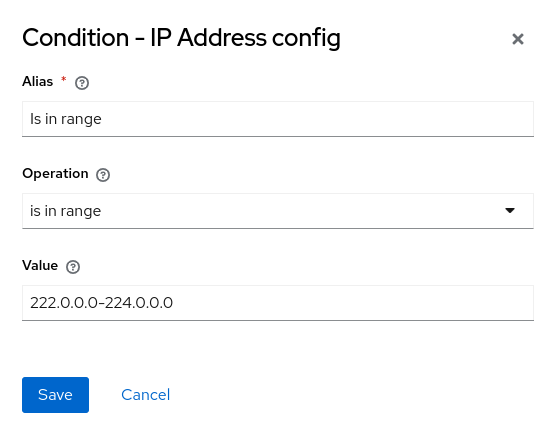
\includegraphics[width=0.8\textwidth]{img/sections/5-design/ip-address-condition.png}
  \label{fig:design-user-context-ip-addr-condition}
  \caption{IP address context condition}
\end{figure}

\section{Authentication Policies} \label{authentication-policies}
Design of the Authentication policies, or as described in the specification as a Policy engine, provides the ability to comply with requirements specified by the administrator.
When users are trying to access the application, they need to meet certain conditions in order to achieve a successful login.
There may be some company or federal restrictions to particular services that need to be conformed to.

For instance, there might be some requirements to deny users access to the application from a specific country or specific types of devices.

It needs to be determined in which authentication process phases these policies should be evaluated.
Policies might be required to comply with some preconditions in order to be able to evaluate them.
It means that the environment context needs to be aligned with the policy requirement, such as gathering information about the user attempting to log in.

A particular hierarchy in policy priorities needs to be assessed as well in order to evaluate specific policies before others.
It provides the capability to create a more complex and comprehensive evaluation pipeline for authentication policies.

Every authentication policy consists of several conditions and actions.
All conditions must be met in order to execute specific actions.
If some of these conditions are not evaluated to be true, the whole authentication policy is skipped, and the following policy in the hierarchy structure is evaluated.

Authentication policies can be specified interactively via the administrator console or HTTP REST API.
All of them are stored in persistent storage, so every change of the structure is visible even after the re-initialization of the application. 
Specific operations can be executed on the policy entities, such as obtaining a specific authentication policy, creating a new one, or updating or removing the existing one.
Moreover, the priority to achieve the required hierarchy structure can be defined as well.

\subsection{Authentication Flow}

Authentication policies are tightly coupled to the authentication flows described in the section \ref{keycloak-authentication-flows}.
Authentication policies are a specific subset of authentication flows as these policies are basically just conditional authentication flows.

Conditional flows provide the majority of the required functionality to meet requirements for authentication policies or the policy engine.
It means that specific conditions are evaluated, and if all pass, specific actions are executed.

One of the major issues around authentication policies is manageability.
Administrators should not add a higher number of conditional flows to their existing authentication flows, as these concepts should be separated in this manner.

Authentication policies extend the capabilities around the authentication flow process as they can be defined for the whole realm, not even for a specific flow.
To be more specific, it gives the possibility to share policies across different flows, which is the main difference between conditional flows and authentication policies.

It provides more fine-grained authentication policy management and a better authentication settings approach.

\subsection{Authentication Policy Authenticator}
In order to properly evaluate all authentication policies specified for the realm without the need to comprehensively expand the authentication flows, a specific authenticator was introduced.
It provides the ability to have a more fine-grained approach for these evaluations, as the administrator can specify in which phases of the authentication flow these policies will be processed.

The authenticator works as a configurable placeholder for these policies, as it can contain multiple configuration properties to asses the overall policies processing.
It might be possible to hide the authenticator from the flows completely, but the explicit settings provide a more deterministic approach.

The default authenticator configuration contains only a boolean flag to determine whether the user information is required for the evaluations or not.

When the authentication flow processing is in the phase of evaluating the authenticator, multiple steps are executed:

\begin{enumerate}
    \item \textbf{Obtain} -- Obtain all authentication policies.
    \item \textbf{Filter} -- Filter policies based on the authenticator configuration.
    \item \textbf{Process} -- Process all authentication policies.
    \item \textbf{Return} -- Return to the parent authentication flow and continue with processing other steps.
\end{enumerate}

When all conditions are met for an arbitrary policy, and the action explicitly allows access to the user, the authenticator itself is evaluated as successful without any other policy evaluations.

The same applies to the case when the action explicitly denies access to the user, the authenticator is evaluated as false, and the whole authentication flow processing is stopped.

Otherwise, when the action is not terminal, the other policies are evaluated as usual.

\subsection{Administrator Console}
// TODO add screenshots of admin pages and elaborate on them

\subsection{Policy Evaluation Example}
For a better representation of the authentication policy evaluation, a simple example with the described configuration might be considered.
The specification of a particular authentication policy is done through the administrator console in the Authentication section and Authentication Policies tab.

The following simple example of the authentication policy, in figure \ref{fig:design-policy-browser-flow}, has one condition and one action.
If the first condition is met, the underlying action is executed.

The policy contains a condition based on the current browser properties, which does not allow a specific browser vendor - Mozilla Firefox, in this case.
When the condition is met, access to the application is denied to the user.
This means that authentication requests can only be made via a browser other than Mozilla Firefox.

\begin{figure}[htbp]
  \centering
  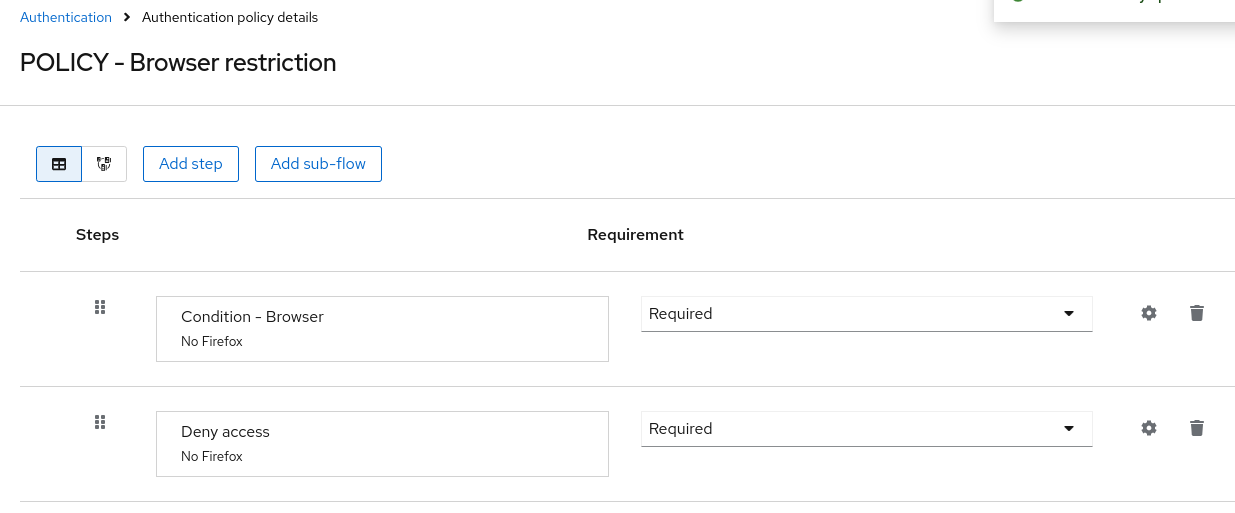
\includegraphics[width=1\textwidth]{img/sections/5-design/policy-browser-flow.png}
  \label{fig:design-policy-browser-flow}
  \caption{Authentication policy browser restriction}
\end{figure}

For a better visualization of the condition evaluation flow, consider this diagram:

\begin{figure}[htbp]
  \centering
  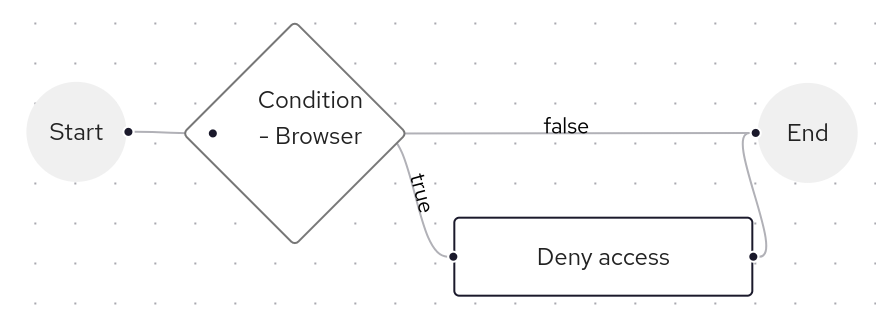
\includegraphics[width=0.8\textwidth]{img/sections/5-design/policy-browser-flow-graph.png}
  \label{fig:design-policy-browser-flow-graph}
  \caption{Authentication policy browser restriction graph}
\end{figure}

The condition configuration attributes differ based on the used condition provider/implementation.
Every condition provider specifies a set of configuration properties for condition settings.

The browser condition, shown in Figure \ref{fig:design-policy-browser-flow-condition}, includes properties:

\begin{itemize}
    \item \textbf{Alias} -- name of the condition.
    \item \textbf{Operation} -- list of possible operations.
    \item \textbf{Browser} -- multi valued list of browsers. 
\end{itemize}

In this case, the condition is met only when the browser vendor is Firefox:

\begin{figure}[htbp]
  \centering
  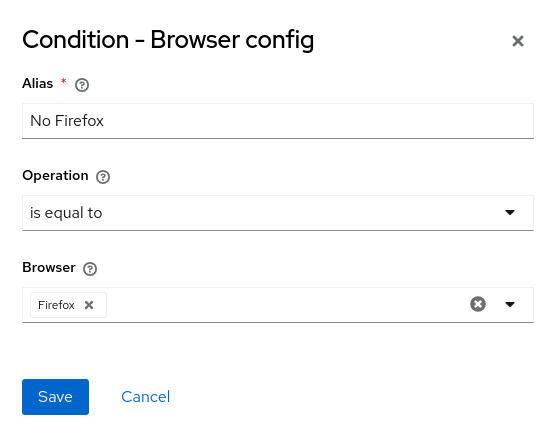
\includegraphics[width=0.8\textwidth]{img/sections/5-design/policy-browser-condition.png}
  \label{fig:design-policy-browser-flow-condition}
  \caption{Browser restriction condition}
\end{figure}

The action configuration also differs based on the provider of the action.
For the Deny access provider, visible in Figure \ref{fig:design-policy-browser-flow-deny}, the only additional property is \textit{Error Message}.
It represents an error message that is shown to the user when the access is denied.

\begin{figure}[htbp]
  \centering
  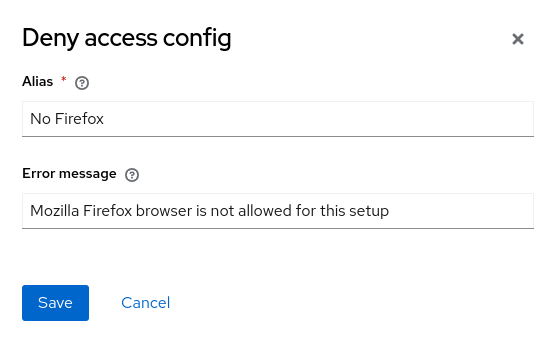
\includegraphics[width=0.8\textwidth]{img/sections/5-design/policy-browser-deny.png}
  \label{fig:design-policy-browser-flow-deny}
  \caption{Browser restriction deny access}
\end{figure}

\newpage
\section{Risk-based Authentication}
The crucial part of adaptive authentication is focused on risk-based authentication.
Risk-based authentication is a concept that assesses a risk level and then adjusts authentication requirements accordingly.
The risk in the risk-based authentication represents a probability that the authentication attempt is fraudulent.
\newline
\newline
The concept is based on this core sequence:
\begin{enumerate}
    \item \textbf{User Context Collection} -- Gather all available user contexts for the following processing. 
    \item \textbf{Risk Scoring} -- Assess the risk score for all the user contexts. 
    \item \textbf{Adaptive Adjustment} -- Adaptively adjust authentication flow based on the overall risk score.
\end{enumerate}

The collection of user contexts is an essential part of the whole risk-based authentication concept - as more information is present, the more informed decisions can be made.
There is a defined timeout for obtaining the user context, as it may take a vast majority of time, and administrators are able to adjust it to their needs.

Obtaining user context from remote locations or services may be time-consuming, and the overall user experience around the authentication process would be worse.
When the timeout is exceeded, the user context is not taken into account for the risk evaluation.

When the user context collection is successful, the risk is evaluated for every user context.
The exact approach and how it is achieved is described in \ref{risk-evaluators}.

When all these evaluations are done, the overall risk for the authentication attempt is calculated with the usage of various algorithms described in \ref{risk-engine}.

After calculating the overall risk, the risk level is determined based on the risk score, described in \ref{risk-levels}.

\newpage
\subsection{Risk Evaluators} \label{risk-evaluators}
Risk evaluators play a crucial role in risk-based authentication, as their primary purpose is evaluating risk for specific user contexts in a fine-grained, modularized way.

The evaluation itself might be a challenging area to handle, as there are no guidelines on how exactly it should be done.
It requires specific expertise and multiple agreements on how exactly the risk should be calculated for each individual user context.

\begin{figure}[htbp]
  \centering
  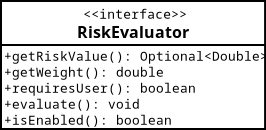
\includegraphics[width=0.4\textwidth]{img/sections/5-design/riskEvaluator.png}
  \label{fig:design-user-evaluator-diagram}
  \caption{Risk Evaluator Diagram}
\end{figure}

\subsubsection{Attributes}
The main risk evaluator attributes:

\begin{itemize}
    \item \textit{risk} -- evaluated risk in range (0,1>.
    \item \textit{weight} -- weight of the evaluated risk in range (0,1> (default 0.5).
    \item \textit{requiresUser} -- flag determining whether the evaluation needs information about the user trying to authenticate. 
    \item \textit{enabled} -- flag determining whether the evaluator risk should be calculated and taken into consideration for the overall risk scoring system. 
\end{itemize}

Attributes \textit{risk} and \textit{weight} contribute to the overall risk scoring system in a magnificent way.
The purpose of the \textit{weight} attribute is to handle every risk evaluation with different weights.
To be more specific, some of these evaluators can contribute more to the overall risk score than others.
It provides the ability to rely on evaluators where the evaluation confidence is higher, and it should influence the overall risk more than evaluators with lower confidence in their evaluations.

Attribute \textit{requiresUser} is a boolean flag used to determine the accurate phase of the evaluation.
Some evaluators need to be already aware of the attempting user, as they need the necessary information about the user.
This means that risk evaluation itself needs to be done after obtaining the essential user information.

Attribute \textit{enabled} is a boolean flag used to check dynamically whether
the evaluator should be turned on.
Administrators can decide which evaluators are taken into account for the processing.

\subsubsection{Scope}
The main risk evaluator characteristic is related to the scope of the user contexts used for these evaluations.
\newline
\newline
Risk evaluators can be determined as:

\begin{itemize}
    \item \textbf{Basic} -- operates only on one user context.
    \item \textbf{Contextual} -- operates on more user context and considers the whole context around obtained specific user contexts.
\end{itemize}

The implementation of a particular risk evaluator should be focused only on one information unit.
It means that in order to provide the fine-grained manageable risk evaluations, the resulting risk should be related only to one user context or component.
In that case, the most suitable approach is to use basic risk evaluators, but sometimes, to properly assess the risk score, a broader context is necessary.

For instance, the risk evaluator handling the calculation of risk for the IP address should be related only to the IP addresses and nothing else.
It may be a contextual risk evaluator, as it needs to obtain device user context, IP address context, or potentially information about proxy usage.
It should not take into consideration a wider context out of its scope as that is not the intentional usage of the component.

For evaluating the overall risk score and considering the wider context, the risk engine component is provided and described in \ref{risk-engine}.

\subsubsection{Configuration}
The key concept around risk evaluators is their configuration for better manageability and user experience.
Administrators have the ability assess the main attributes of evaluators to their needs, such as tweaking the \textit{weight} or \textit{enabled} attribute without the necessity to change the risk evaluators implementation.

In the \textit{Risk-based policies} section of the administrator console, properties for value amendment are automatically generated.
When a developer creates another risk evaluator, the configuration for the basic configurable attributes is generated in the administrator console.

As shown in the figure \ref{fig:risk-based-evaluator-config}, the risk evaluators configuration contains multiple similar configuration fields grouped together, and noted via the colored rectangles. 

\begin{figure}[htbp]
  \centering
  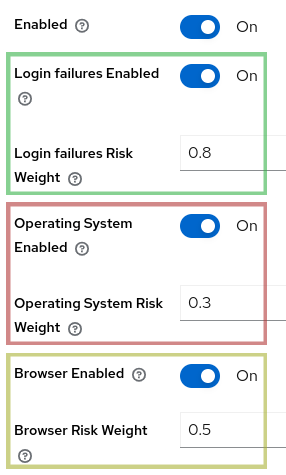
\includegraphics[width=0.5\textwidth]{img/sections/5-design/risk-evaluators-config.png}
  \label{fig:risk-based-evaluator-config}
  \caption{Risk Evaluators Configuration}
\end{figure}

\newpage
\subsection{Risk Engine} \label{risk-engine}
The risk engine takes care of evaluating the overall risk score based on scores obtained from the risk evaluators.
One of the primary purposes of the risk engine is to manage the underlying evaluators, such as processing their lifecycle phases and contextually evaluate the overall score.

Each implementation can provide its own approach to send signal to evaluators to start evaluating risk scores or specify a different algorithm for the overall risk score.

The default risk engine provides a retry mechanism when the risk evaluator does not return any result.
Failure may occur when obtaining the user context or evaluating the risk score.
It is usually a problem of leveraging remote services, as the process is more comprehensive and includes several additional potential points of failure.
When the processing fails, the risk engine requests to retry the evaluation again.

The default risk engine also introduces a timeout mechanism as the delivery time is guaranteed and upper bounded.
Expressly, it is guaranteed that processing the risk for individual evaluators does not exceed the defined timeout and does not allocate the processor timeout with the following application unresponsiveness.

The overall risk score is evaluated continuously based on the phase of authentication.
During the authentication flow, the risk may be evaluated multiple times, as the requirements for the risk evaluators and risk engine context may differ.
The fundamental phases of risk engine evaluation are \textit{NO\_USER} and \textit{REQUIRES\_USER}. 

The \textit{NO\_USER} phase represents the phase before determining who is trying to access the application.
It means only information about the application stack is present, such as information about the device and network.

The \textit{REQUIRES\_USER} phase represents the phase when the user is already known during the authentication process.

\subsubsection{Default Algorithm}
The default algorithm for calculating the overall risk score is weighted arithmetic mean, which provides the necessary characteristic for the risk evaluation.

The weighted arithmetic mean shares similarities with the standard arithmetic mean, the typical average calculation method.
However, unlike the arithmetic mean, where each data point holds equal weight in determining the final average, the weighted arithmetic mean assigns varying weights to different data points.

This is an exact concept suitable for leveraging risk evaluators and aggregating their results.
When all weights are uniform, the weighted mean converges to the arithmetic mean.
\newline
\newline
Formula for the weighted arithmetic mean:
\begin{equation}
\bar{x} = \frac{\sum_{i=1}^{n} w_i \cdot x_i}{\sum_{i=1}^{n} w_i}
\end{equation}

The \( \bar{x} \) represents the overall risk score, \( x_i \) represents the individual risk evaluator score, and \( w_i \) represents the corresponding weight for each risk evaluator.

The overall risk of the whole authentication process is evaluated as an arithmetic average of risk scores for each individual phase.
It means when the overall score for phase \textit{NO\_USER} is \textit{0.7}, and the score for phase \textit{REQUIRES\_USER} is \textit{0.6}, the overall risk score for the whole process is \textit{0.65}. 

\subsubsection{Design}
The risk engine is presented as \textit{RiskEngine} interface with several methods shown in Figure \ref{fig:design-user-engine-diagram}.
The interface extends \textit{ConfigurableRequirements} interface for achieving dynamic check whether the authentication user is required during the risk engine processing.
There is also a weak relationship between \textit{RiskEngine} and \textit{RiskEvaluator} interface, as \textit{RiskEngine} contains collection of the risk evaluators.
Therefore the aggregation relationship is used in this case. 
\newline
\newline
Risk engine methods:

\begin{itemize}
    \item \textit{evaluateRisk()} -- method that initiates the evaluation of the collected risk.
    \item \textit{getRisk()} -- retrieve the evaluated risk.
    \item \textit{getRiskEvaluators()} -- retrieve all risk evaluators that contribute to the risk calculations.
\end{itemize}

\begin{figure}[htbp]
  \centering
  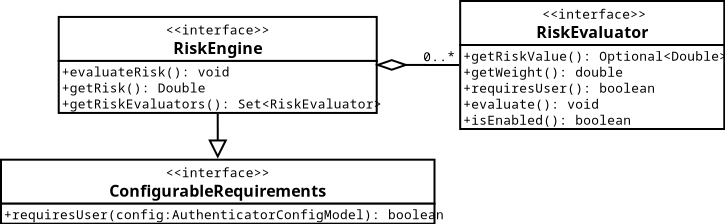
\includegraphics[width=1\textwidth]{img/sections/5-design/risk-engine.png}
  \label{fig:design-user-engine-diagram}
  \caption{Risk Engine Diagram}
\end{figure}

\subsubsection{Configuration}
It is essential for administrators to have the capability to set reasonable values for the timeout and number of retries for the risk engine.
Besides configuring the overall state of risk-based functionality, it may be done through the administrator console, as shown in figure \ref{fig:risk-based-enging-config}.
The default number of retries is \textit{3}.
The default timeout for processing the risk score is \textit{1500ms}.

\begin{figure}[htbp]
  \centering
  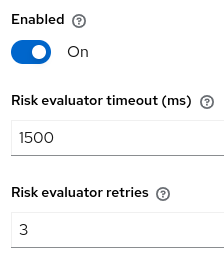
\includegraphics[width=0.4\textwidth]{img/sections/5-design/risk-based-engine-config.png}
  \label{fig:risk-based-enging-config}
  \caption{Risk Engine Configuration}
\end{figure}

\subsubsection{Stored Risk Provider}
As the overall risk score is evaluated in several phases, the results for every phase need to be available in some manner. 
The most reasonable approach would be storing the data in a particular place for later processing.

The lifespan of these data should not exceed the lifespan of the authentication request.
However, when some action is required from the user, such as providing a password, the HTTP and authentication requests are different.

The start for the authentication request might be considered at the beginning of processing the authentication flow when the Keycloak authentication session is created.
Therefore, leveraging authentication session notes seems to be the most reasonable way to store the risk.

However, these data might be stored in different stores, such as databases or cache, and the developer should have the ability to extend the functionality.
Thus, the \textit{SPI} for the stored risk is introduced.
The provider for storing the risk is represented by \textit{StoredRiskProvider}, shown in Figure \ref{fig:design-stored-risk-diagram}.

\begin{figure}[htbp]
  \centering
  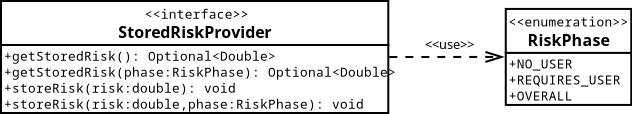
\includegraphics[width=1\textwidth]{img/sections/5-design/stored-risk-provider.png}
  \label{fig:design-stored-risk-diagram}
  \caption{Stored Risk Provider Diagram}
\end{figure}

Stored risk provider methods:
\begin{itemize}
    \item \textit{getStoredRisk()} -- retrieve the overall stored risk score.
    \item \textit{getStoredRisk(phase)} -- retrieve the risk score for specific risk phase.
    \item \textit{storeRisk(risk)} -- store overall risk score.
    \item \textit{storeRisk(risk, phase)} -- store risk score for specific risk phase.
\end{itemize}

Risk phase values representing the phase of the evaluated risk score are detailed described in the general subsection of \ref{risk-engine}.

\subsubsection{Risk Engine Authenticator}
The primary purpose of the risk engine authenticator is to explicitly trigger the risk engine evaluations for specific risk processing phases.
It is the standard Keycloak authenticator so that it can be included in a specific place in an authentication flow.
The intention behind introducing the authenticator is to have better control over the risk processing lifecycle without the need to touch the Keycloak codebase out of the Keycloak extension.

It might be possible to hide the authenticator for administrators, as it would be evaluated once the risk processing phase met some specific condition that checks the ability to process it.
\newline
\newline
The authenticator configuration looks like this:

\begin{figure}[htbp]
  \centering
  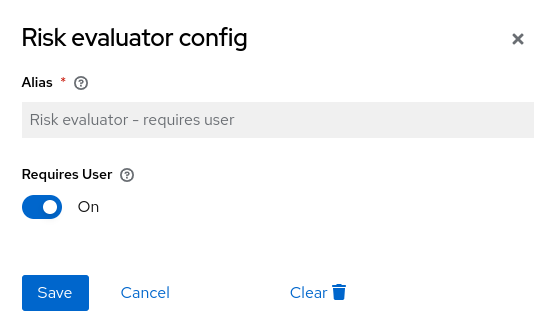
\includegraphics[width=0.8\textwidth]{img/sections/5-design/risk-evaluator-authenticator-config.png}
  \label{fig:risk-evaluator-authenticator-config}
  \caption{Risk Engine Authenticator Configuration}
\end{figure}

\subsection{Risk Levels} \label{risk-levels}
When the risk engine calculates the overall risk score for the authentication request, the application needs to react to it in some manner.
The primary purpose of the risk levels is to divide risk score ranges into specific levels.
The risk level is basically an entity with a specified lower and upper bound of risk score shown in Figure \ref{fig:risk-level-diagram}.

\begin{figure}[htbp]
  \centering
  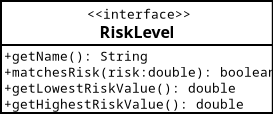
\includegraphics[width=0.45\textwidth]{img/sections/5-design/risk-level.png}
  \label{fig:risk-level-diagram}
  \caption{Risk Level Diagram}
\end{figure}

Risk level methods:
\begin{itemize}
    \item \textit{getName()} -- retrieve the name of the level.
    \item \textit{matchesRisk(risk)} -- check whether a specific risk is associated to a risk level.
    \item \textit{getLowestRiskValue()} -- retrieve the lower risk bound.
    \item \textit{getHighestRiskValue()} -- retrieve the upper risk bound.
\end{itemize}

As the risk score might consider dynamic evaluations, which can provide slightly different fluctuating results, relying on specific risk score values is impossible.
That means a reasonable granularity needs to be assessed to manage the overall risk score -- several levels.
There are two default distinct risk level categories providing different granularity of risk levels -- \textit{simple} and \textit{advanced}.
Developers can provide their custom risk level category by implementing the \textit{RiskLevelsSpi}.
\newline
\newline
The \textit{simple} risk level category consists of three risk levels:
\begin{itemize}
    \item \textbf{Low} -- Risk score in range (0, 0.33>.
    \item \textbf{Medium} -- Risk score in range (0.33, 0.66>.
    \item \textbf{High} -- Risk score in range (0.66, 1>.
\end{itemize}
\newline
\newline
The \textit{advanced} risk level category consists of five risk levels:
\begin{itemize}
    \item \textbf{Low} -- Risk score in range (0, 0.2>.
    \item \textbf{Mild} -- Risk score in range (0.2, 0.4>.
    \item \textbf{Medium} -- Risk score in range (0.4, 0.6>.
    \item \textbf{Moderate} -- Risk score in range (0.6, 0.8>.
    \item \textbf{High} -- Risk score in range (0.8, 1>.
\end{itemize}

\begin{figure}[htbp]
  \centering
  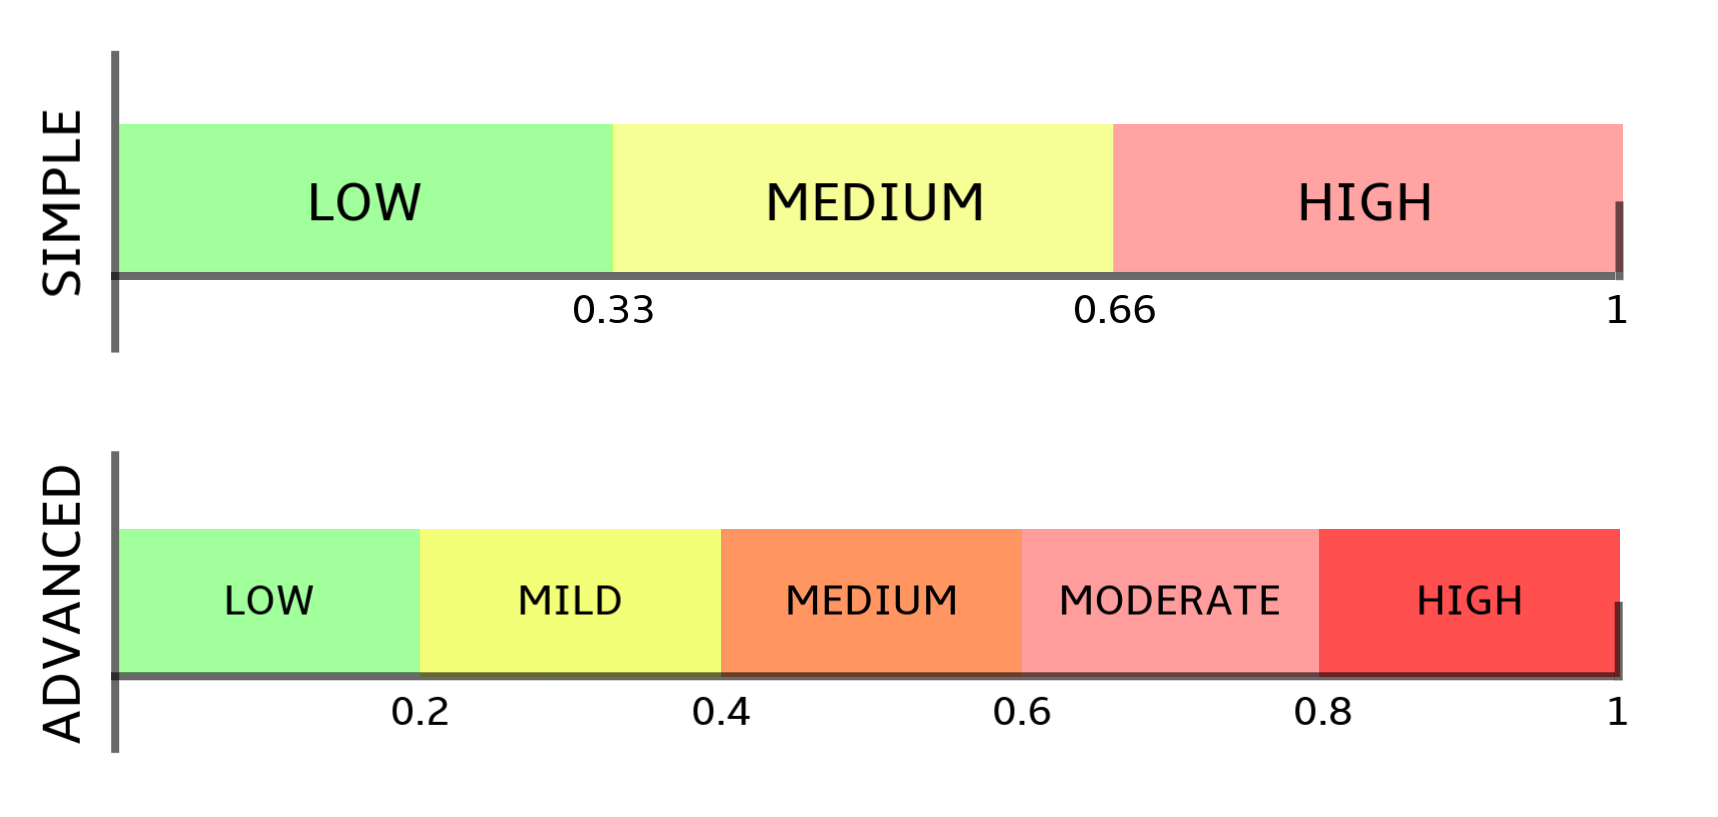
\includegraphics[width=1\textwidth]{img/sections/5-design/risk-levels.png}
  \label{fig:risk-levels}
  \caption{Default Risk Levels}
\end{figure}

\subsubsection{Risk Level Conditions}
In order to accommodate the risk levels mechanism into the authentication flow, expressly conditional flows or authentication policies, the risk level condition is introduced.
The primary purpose of the condition is to process conditional flow or authentication policy when its predicate is evaluated as \textit{true}.

In this case, the predicate obtains the stored risk from the risk engine and, based on the specified risk level category, determines whether the risk is included in the risk level category.
If the evaluated risk score is in the range of the specified category, the condition is evaluated as \textit{true}, and the underlying flow is processed.
\newline
\newline
The list showed to administrators when adding a condition to the conditional flow or authentication policies:

\begin{figure}[htbp]
  \centering
  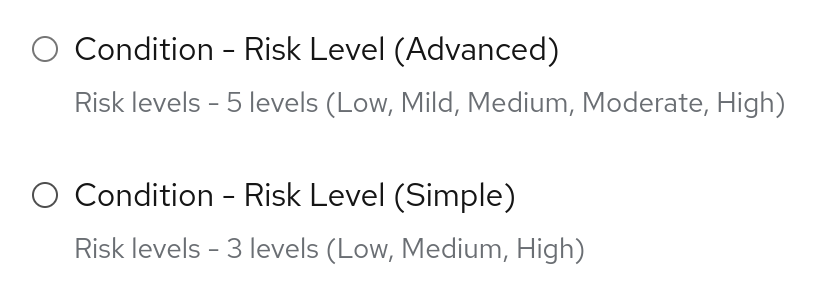
\includegraphics[width=0.7\textwidth]{img/sections/5-design/risk-level-condition-list.png}
  \label{fig:risk-levels-condition}
  \caption{Default Risk Levels Condition}
\end{figure}

The risk level condition contains a configuration list box with values defined for the particular risk level provider, as shown here:

\begin{figure}[htbp]
  \centering
  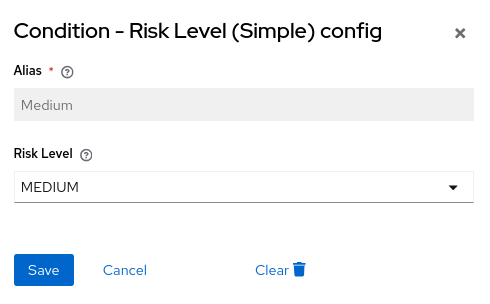
\includegraphics[width=0.8\textwidth]{img/sections/5-design/risk-level-simple-config.png}
  \label{fig:risk-levels-simple-config}
  \caption{Simple Risk Level Configuration}
\end{figure}

\subsubsection{Risk Level Flow Example}

A proper example of leveraging the risk levels in the conditional flows or authentication policies might be seen in Figure \ref{fig:risk-levels-example} below.
The risk level flow is a sequence of conditional flows consisting of risk level conditions and actions that should be executed.
For better visibility, the conditional flows are marked by different colors.
\newline
\newline
In the case shown in Figure \ref{fig:risk-levels-example}, consider the \textit{simple} risk level category. When the evaluated risk is:
\begin{itemize}
    \item \textbf{Low} -- the access to the application is granted without any other action.
    \item \textbf{Medium} -- the second factor is required -- using OTP.
    \item \textbf{High} -- the access is denied.
\end{itemize}

\begin{figure}[htbp]
  \centering
  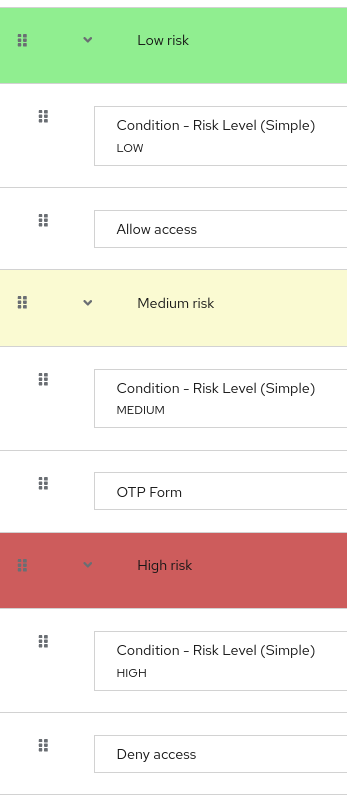
\includegraphics[width=0.5\textwidth]{img/sections/5-design/simple-risk-level-flow.png}
  \label{fig:risk-levels-example}
  \caption{Simple Risk Level Flow}
\end{figure}


\newpage
\section{Artificial Intelligence}

\newpage
\section{External Integration}